\begin{frame}{Design fra CBF's}{Use-cases og fælles udfordringer}
\section{Design fra CBF's}
\begin{minipage}{0.5\textwidth}
	\begin{block}{Tre use-cases}
		\begin{itemize}
			\item Et "simpelt" case i 1D \\ \scriptsize{ - skabe erfaring med CBF's og den anvendte kontrol topologi}
			\item  \normalsize Virtual fixture \\ \scriptsize - at starte noget virkeligt anvendeligt
			\item \normalsize  Operationer i 3D rummet \\  \scriptsize - undgå at bringe vitale områder i fare
		\end{itemize}
	\end{block}
	\begin{block}{Fælles udfordringer\\ \scriptsize {\color{white}{lol}} - som vi møder som de første i Danmark}
		\begin{itemize}
			\item Konstruktion af CBF's \\ \scriptsize - som at lede efter Lyapunov funk.
			\item \normalsize Kontrol topologi
			\item Implementering på da Vinci med ROS
		\end{itemize}
	\end{block}
\end{minipage}
\hspace{0.3cm}
\begin{minipage}{0.45\textwidth}
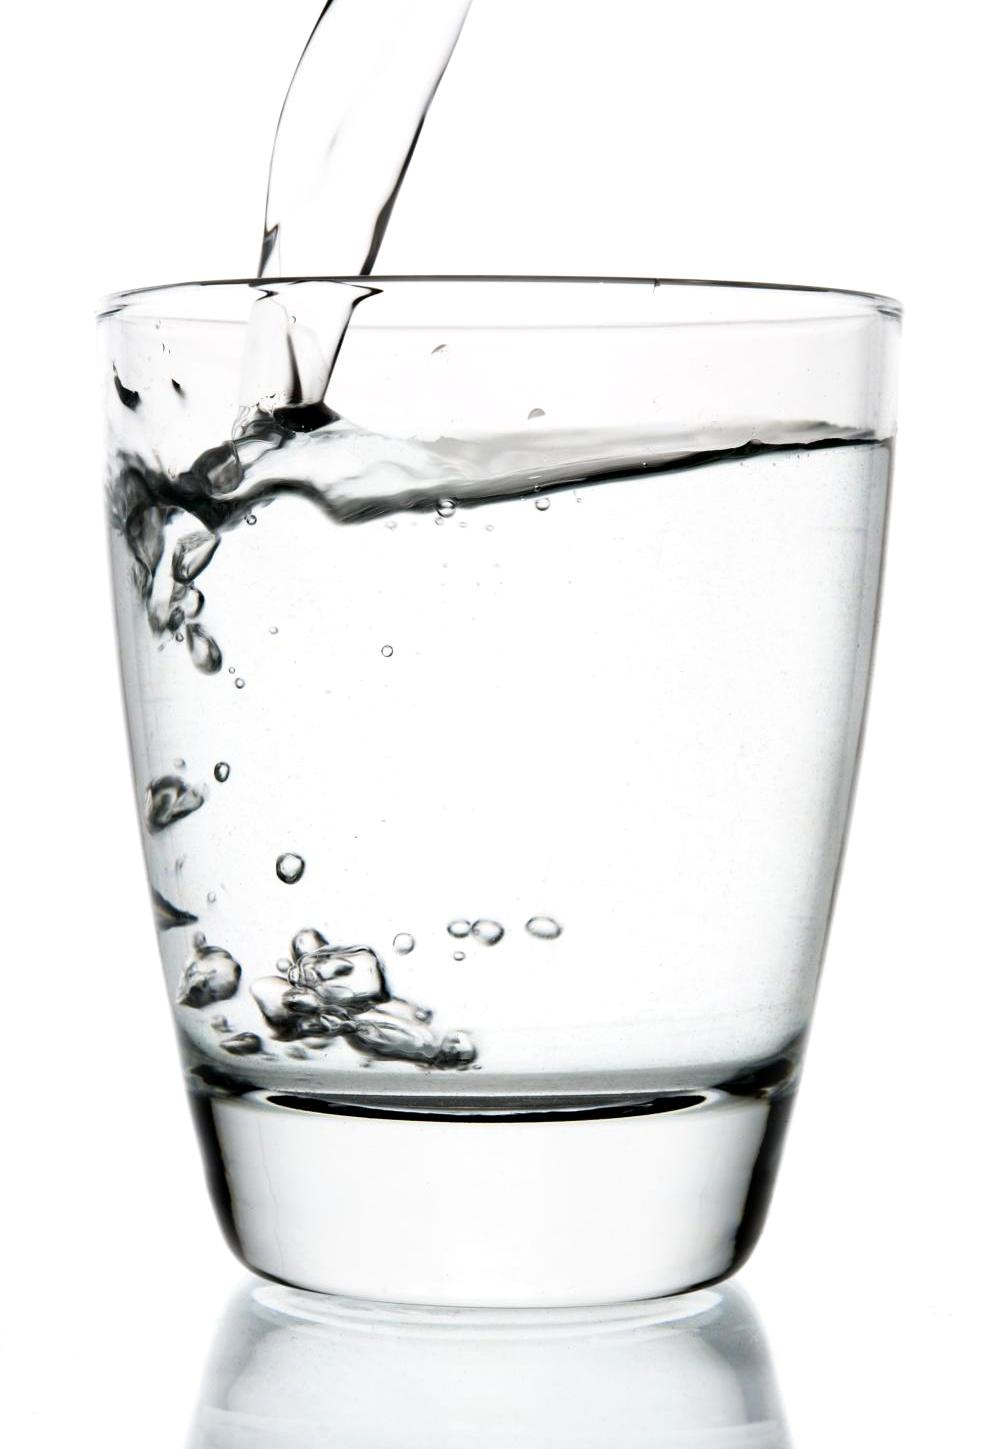
\includegraphics[width=0.35\linewidth]{simple}
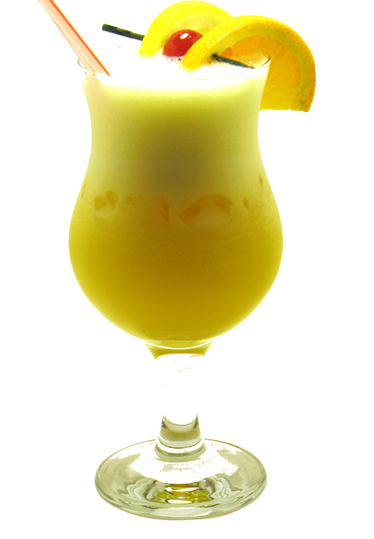
\includegraphics[width=0.35\linewidth]{tri.png}
\vspace{0.2cm}
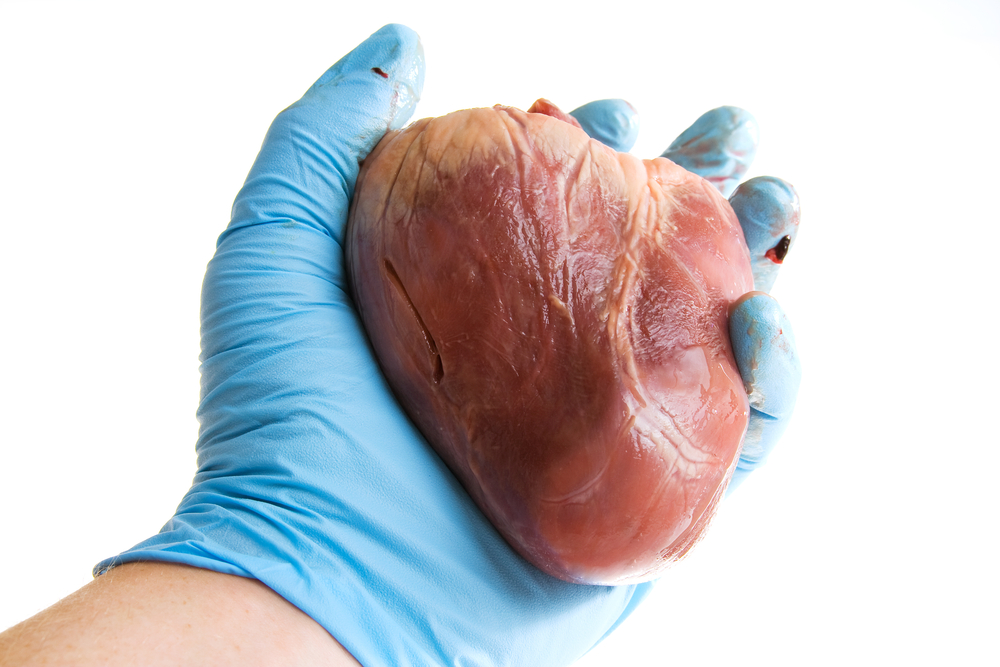
\includegraphics[width=0.6\linewidth]{human-heart.jpg}
\vspace{0.2cm}
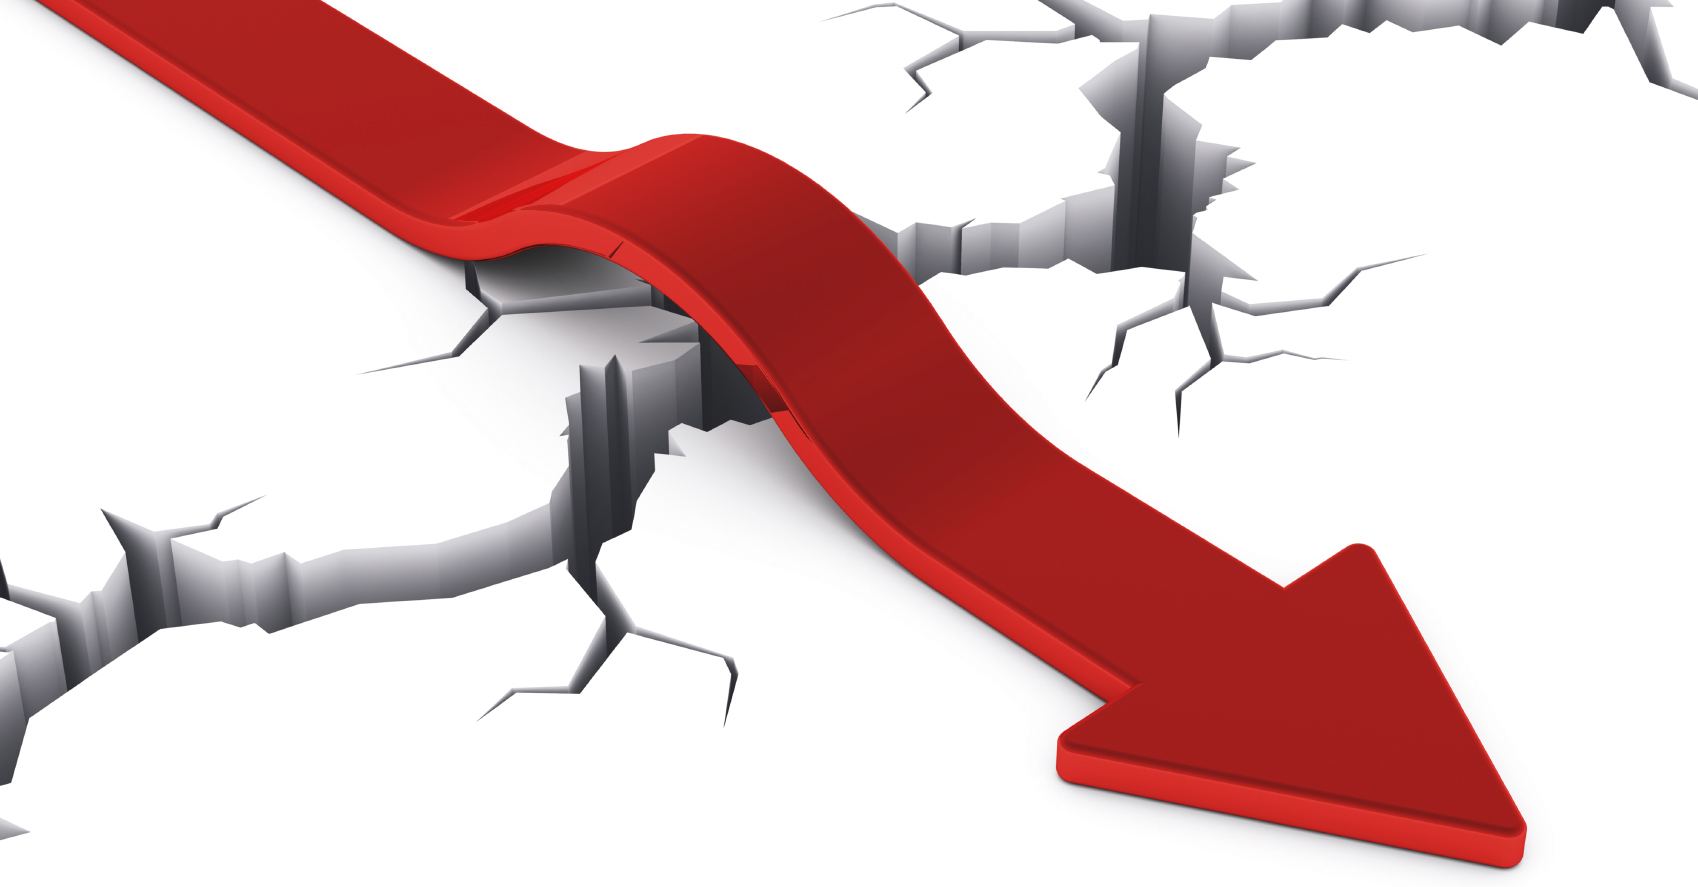
\includegraphics[width=0.8\linewidth]{SIIB.jpg}
\vspace{0.2cm}
\end{minipage}
\end{frame}

\begin{frame}{Sikkerhed for et 1 dimensionelt system}{Det første skridt - instrument slide}
\section{Sikkerhed i 1D}
\vspace*{-0.5cm}
\begin{minipage}{0.6\textwidth}
\begin{block}{}
	\begin{itemize}
		\item Model
		\begin{itemize}
			\item 1. orden: Opnå erfaring
			\item 2. orden: Observer krævet
		\end{itemize}
		\item CBF
		\begin{itemize}
			\item parabel for 1. orden
			\item paraboloid for 2. orden
		\end{itemize}
			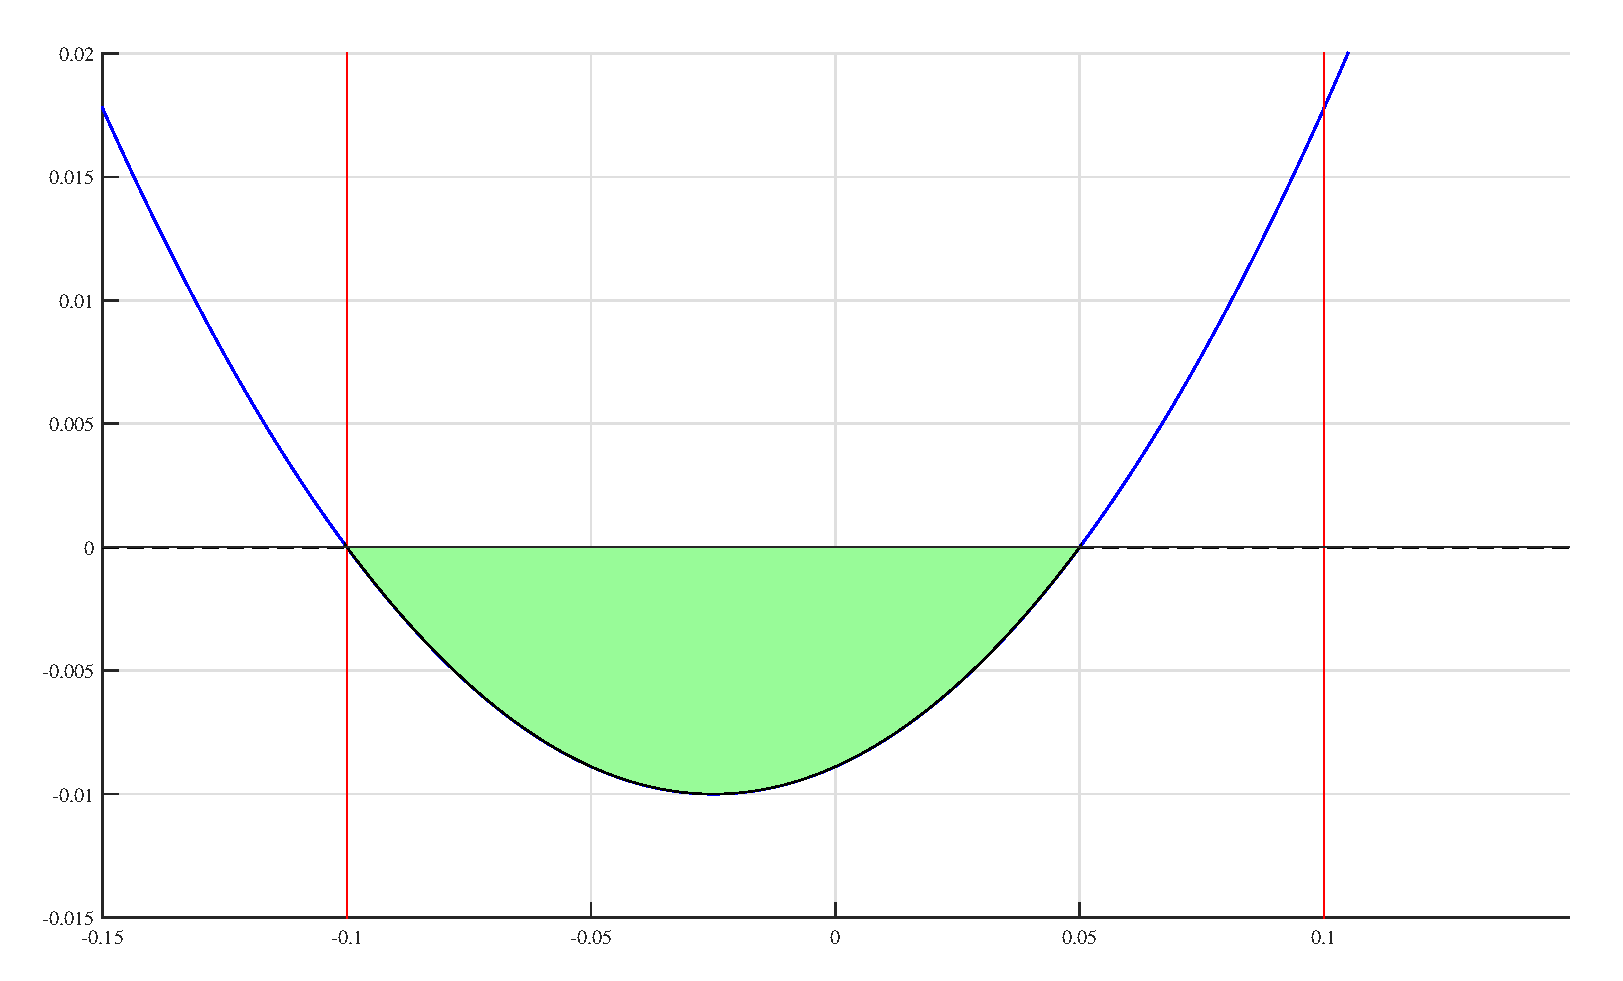
\includegraphics[width=0.4\linewidth]{cbf_1d.eps} \hspace{0.2cm}
			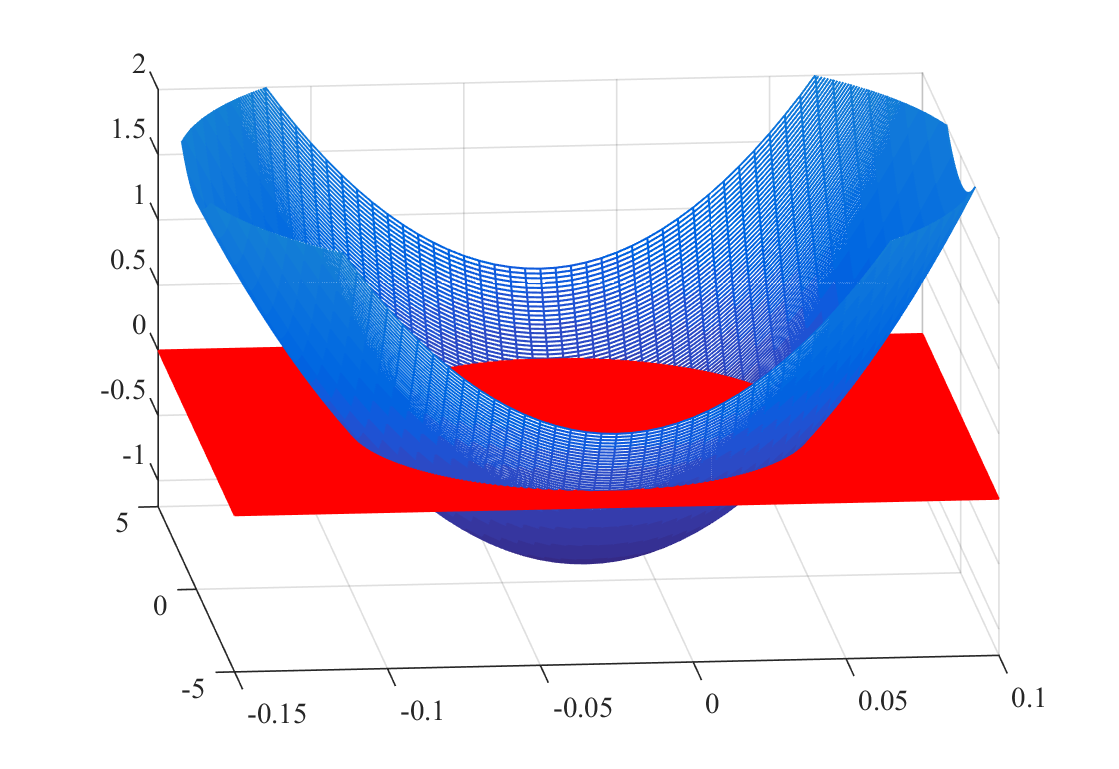
\includegraphics[width=0.4\linewidth]{cbf_2d.eps}
		\item Simulering med Forward Euler
	\end{itemize}
\end{block}
\vspace{-0.7cm}
\scriptsize
\begin{align*}
&\scriptsize \dot{x} = \lambda x \nonumber \\
&\dot{x} = \frac{x_n - x_{n-1}}{t_n - t_{n-1}} = \frac{x_n - x_{n-1}}{h} = \lambda x_{n-1}  \\
& x_n = x_{n-1}(1+h\lambda) = x_0(1+h\lambda)^n \\
&\Rightarrow \,\,\, |1+h\lambda| > 1 \,\,\,\text{ustabil} 
\end{align*}
\end{minipage}
\hspace{0.3cm}
\begin{minipage}{0.35\textwidth}
{\color{white}{white}}\\
{\color{white}{white}}
\hspace*{-0.5cm}
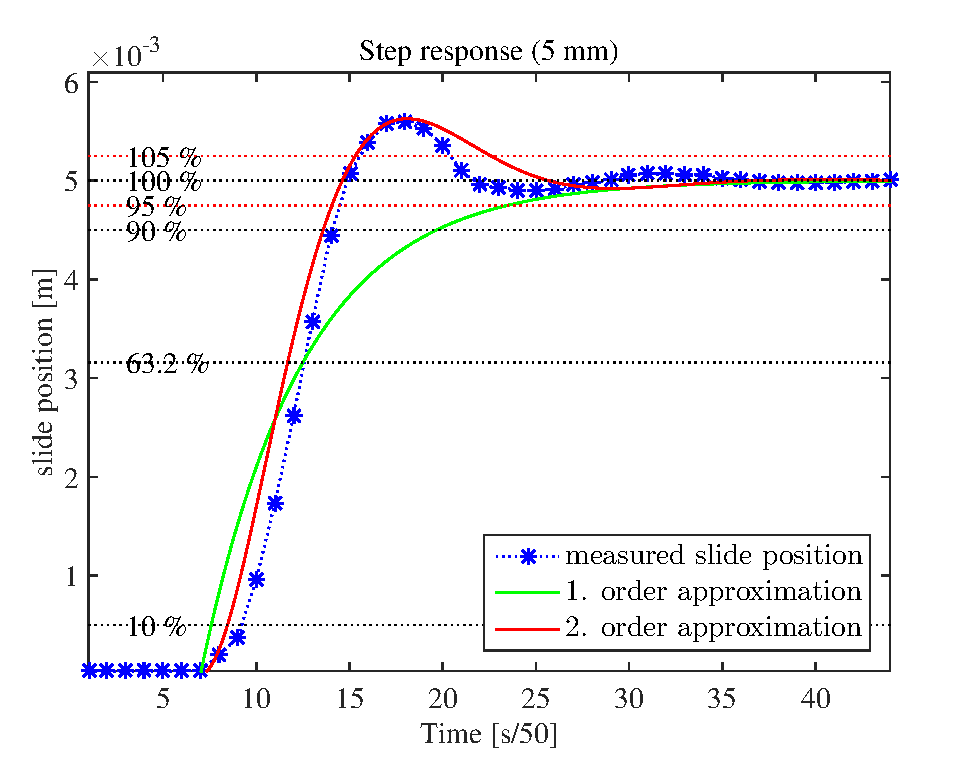
\includegraphics[width=1.1\linewidth]{model_1d.eps}

\hspace*{-0.5cm}
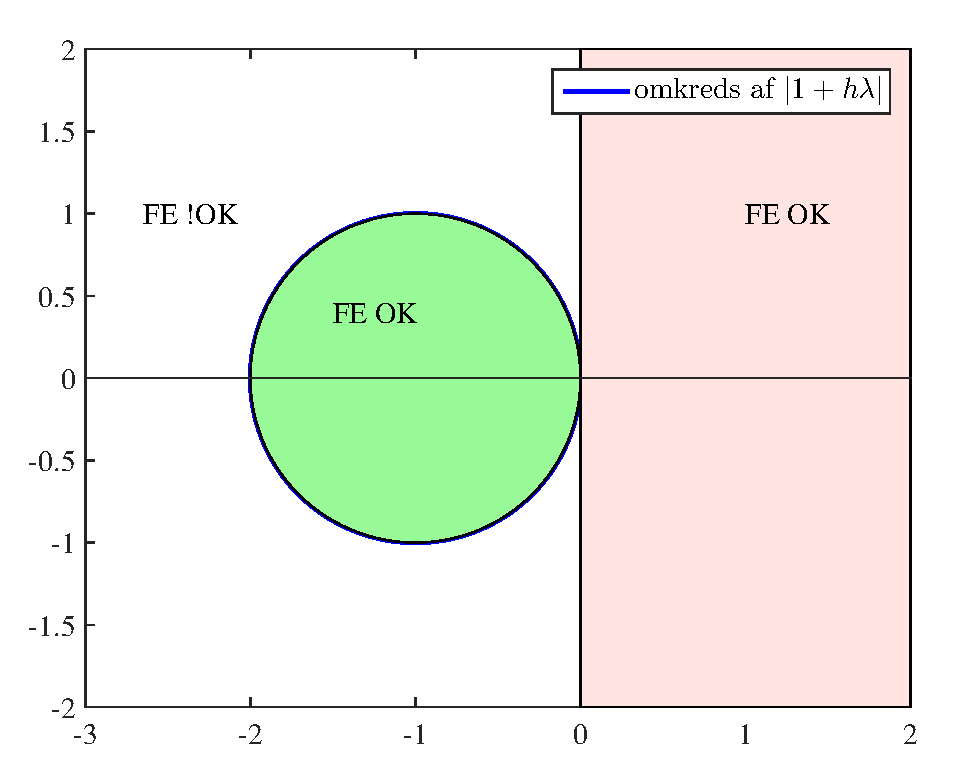
\includegraphics[width=1.1\linewidth]{fe_graphs.eps}

\end{minipage}
\end{frame}


\begin{frame}{Sikkerhed for et 1 dimensionelt system}{Resultater og erfaring}
\begin{minipage}{0.48\textwidth}
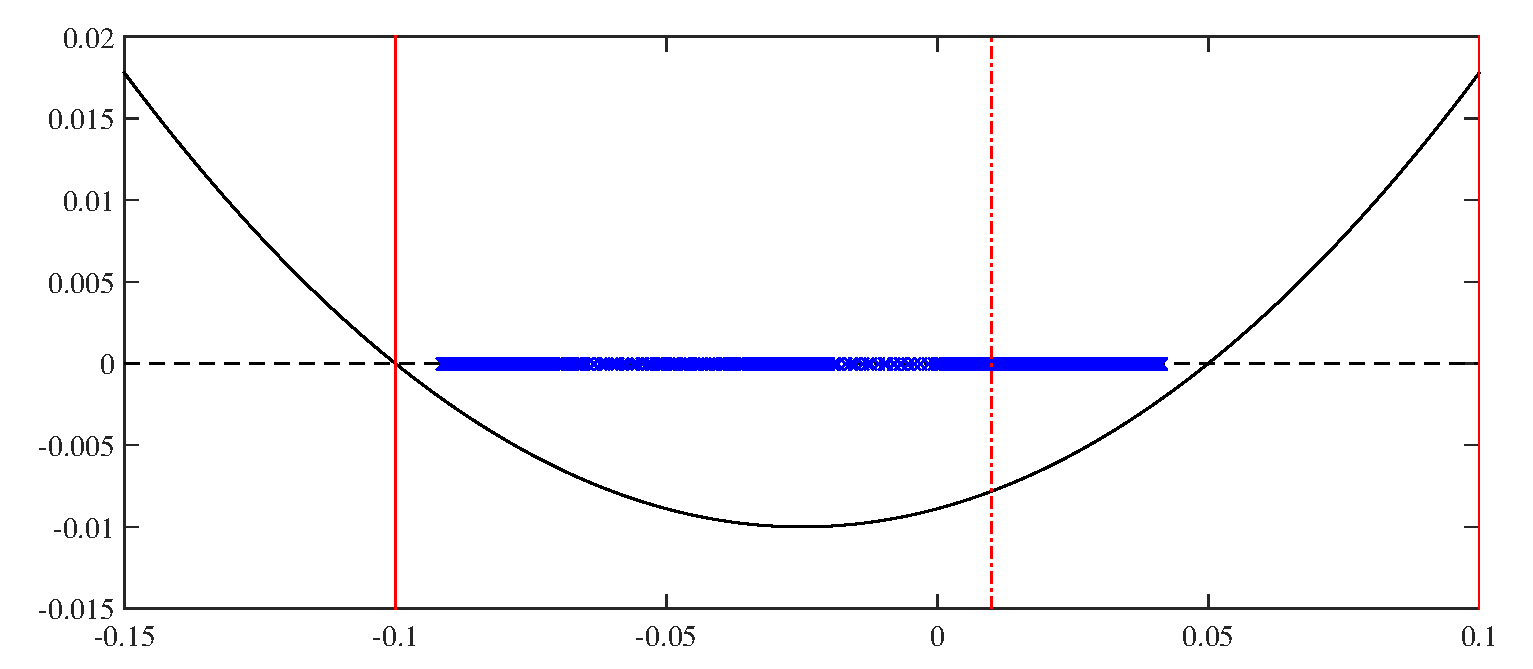
\includegraphics[width=1\linewidth]{plot_states_nem.eps}

\begin{itemize}
%	\item \scriptsize $\tilde{u}(\textbf{x},u) = k_0(\textbf{x})\sigma(\textbf{x}) + ( 1-\sigma(\textbf{x}) ) u(\textbf{x})$
	\item \scriptsize $k_0(\textbf{x}) = -\dfrac{a + \sqrt{a^2 + \kappa^2 b b^T}}{b b^T} b^T$
%	\item \scriptsize $\sigma(\textbf{x}) = \begin{cases} 1 \\ \text{bump function} \\ 0 \end{cases}$
%	\item Betydning af $\kappa$, $\sigma$, ..
%	\item simulering + da Vinci implementering
\end{itemize}


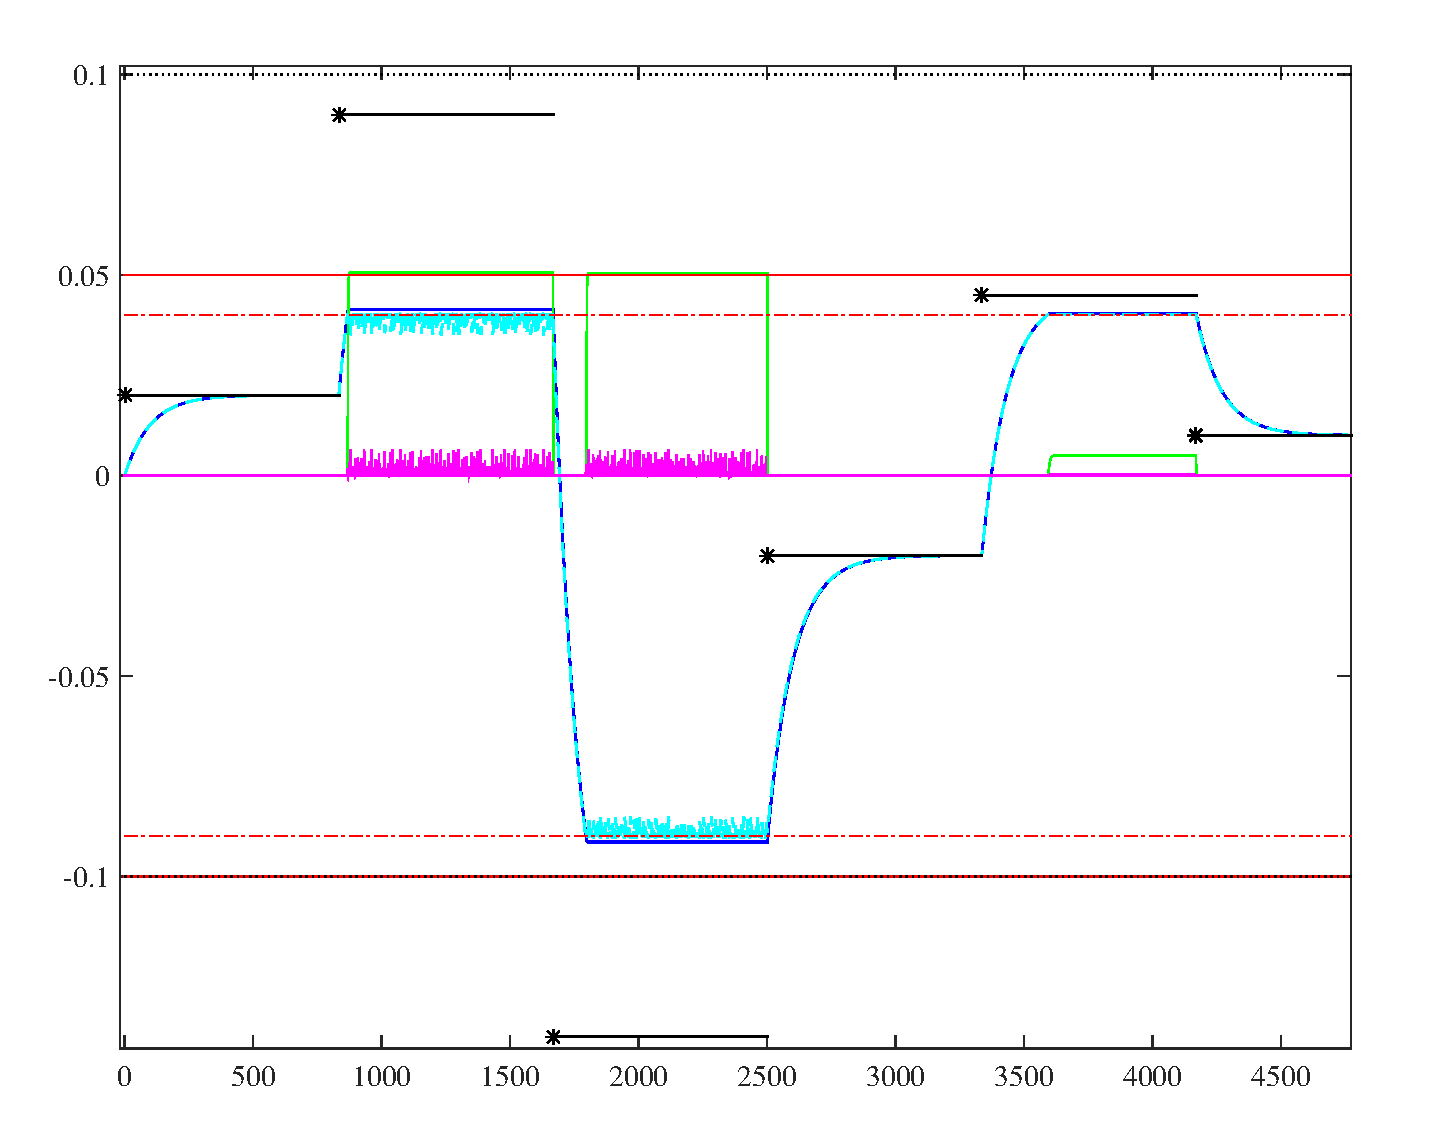
\includegraphics[width=1\linewidth]{vary_kappa.eps}
\vspace*{-0.4cm}


\end{minipage}
\begin{minipage}{0.48\textwidth}
{\color{white}{white}}
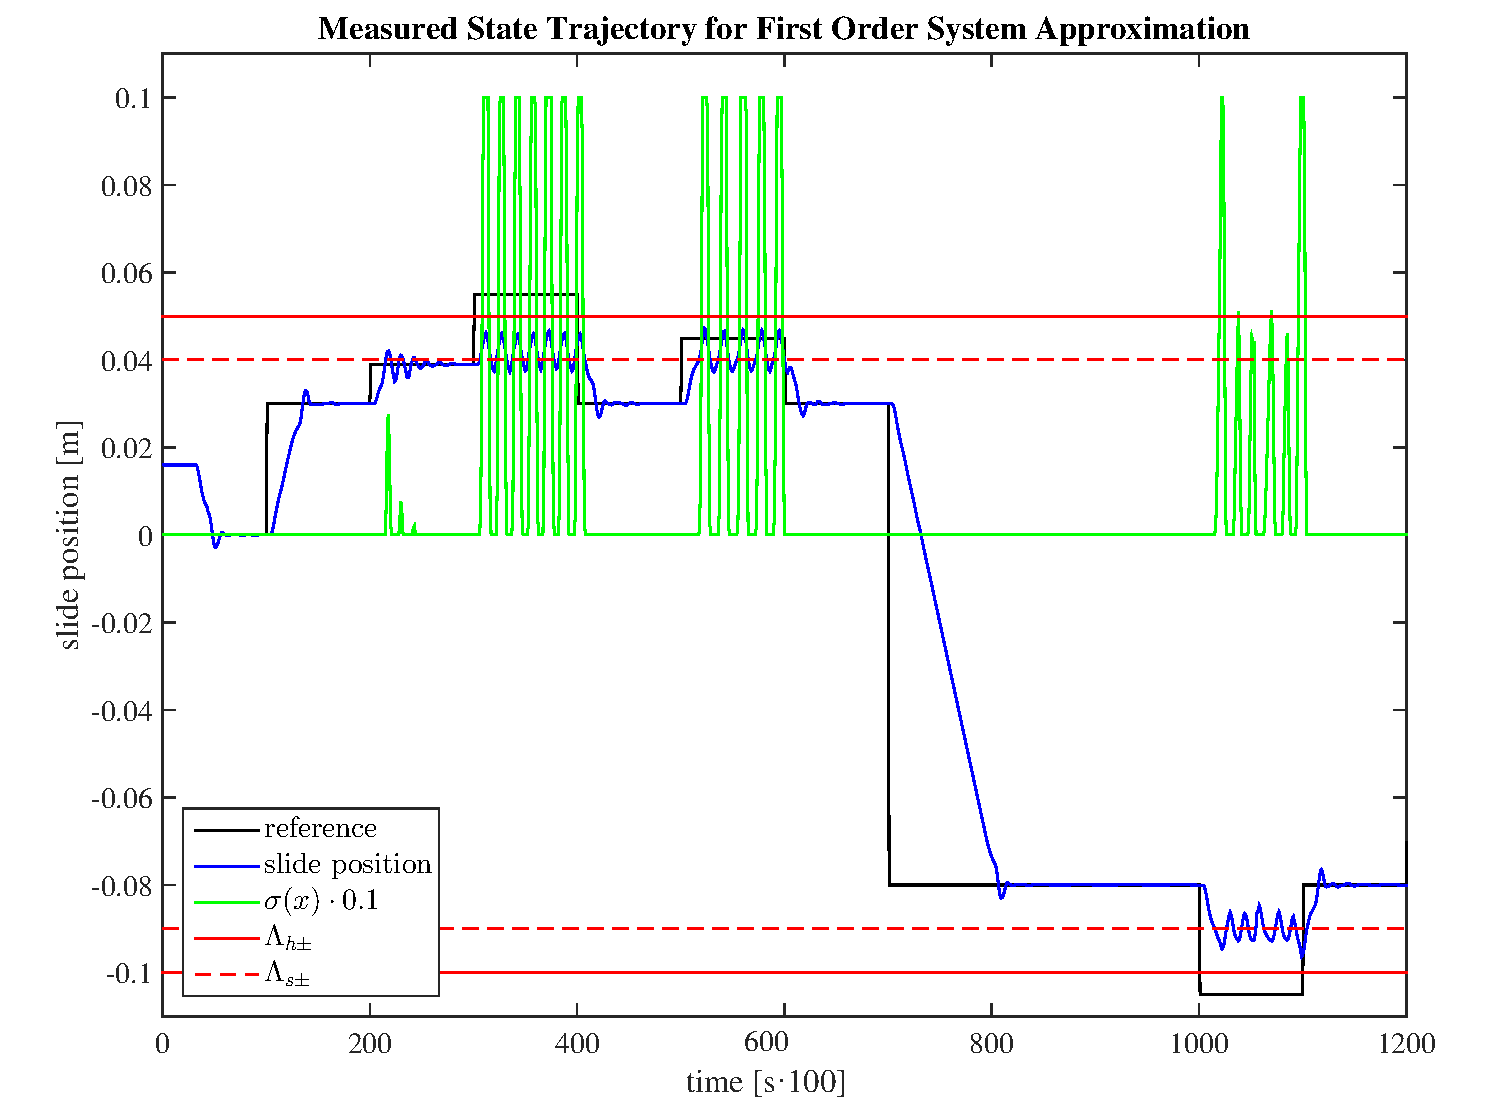
\includegraphics[width=1\linewidth]{trajectory_slide_meas_1-eps-converted-to.pdf}

\vspace*{0.05cm}
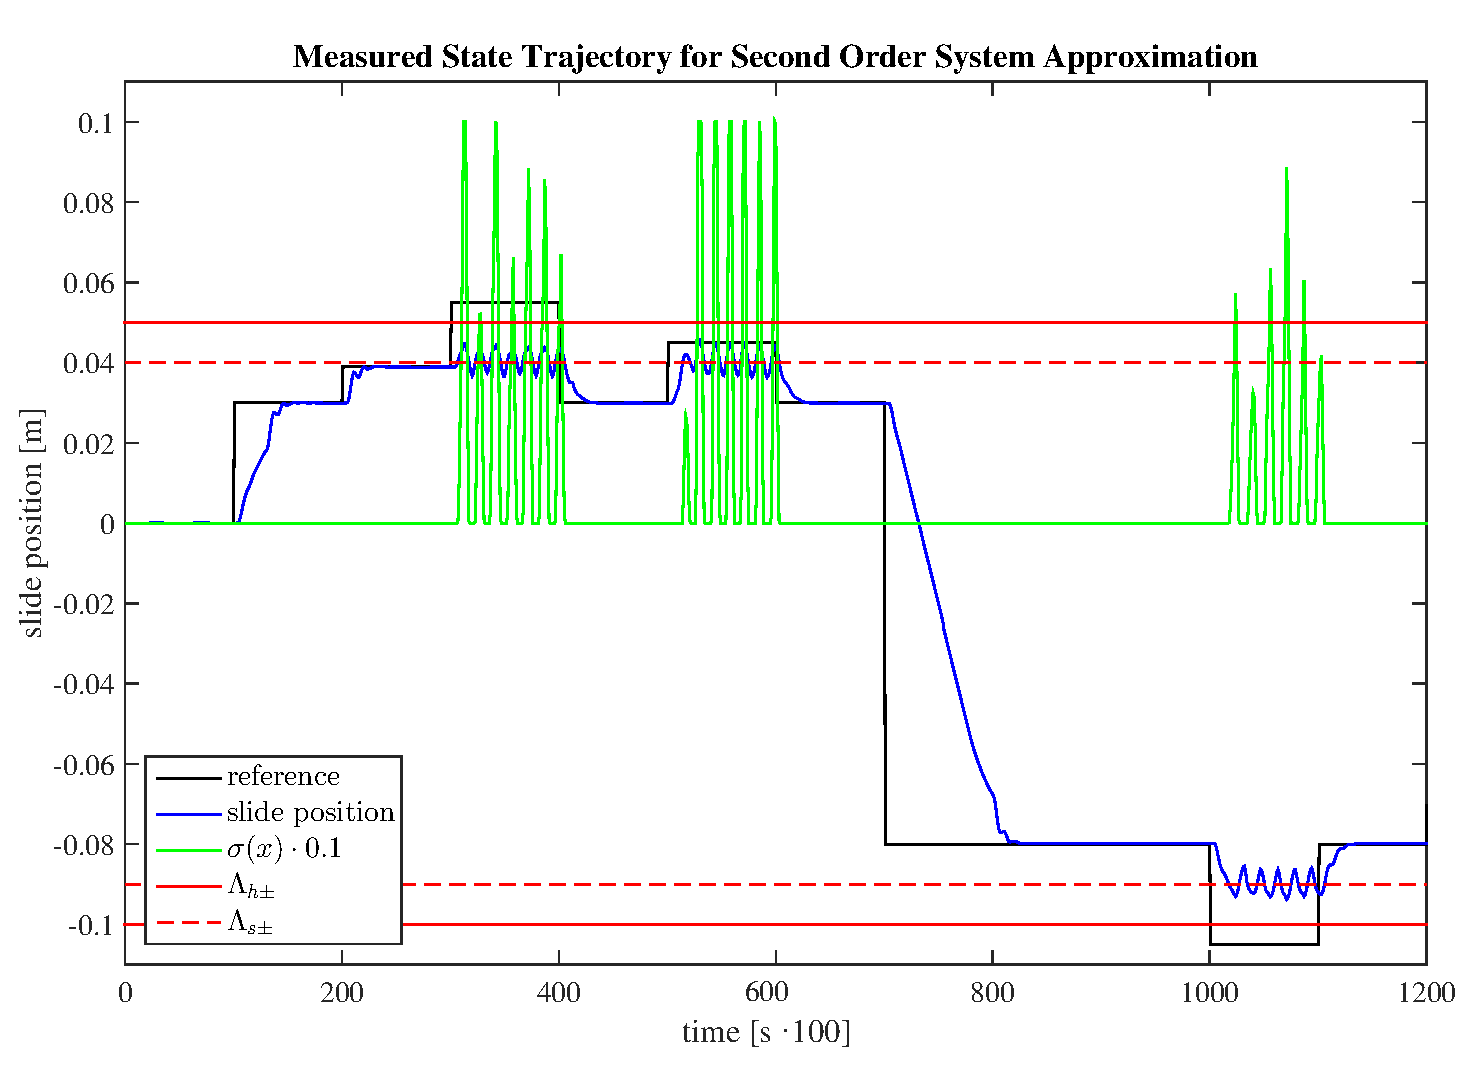
\includegraphics[width=1\linewidth]{meas_trajectory_2_order-eps-converted-to.pdf}

\end{minipage}
\end{frame}

\begin{frame}{Sikkerhed for et dynamisk system}{Indledende udvikling til at opnå virtual fixture}
\section{Virtuel fixture}
\vspace*{-0.7cm}
\begin{block}{}
	\begin{itemize}
		\item Opnå en sikker afstand
		\item Lægen skal opleve hjertet som stillestående
		\item Modeller hjertet som en sinus bevægelse (Dr. Poulsen)
	\end{itemize}
\end{block}
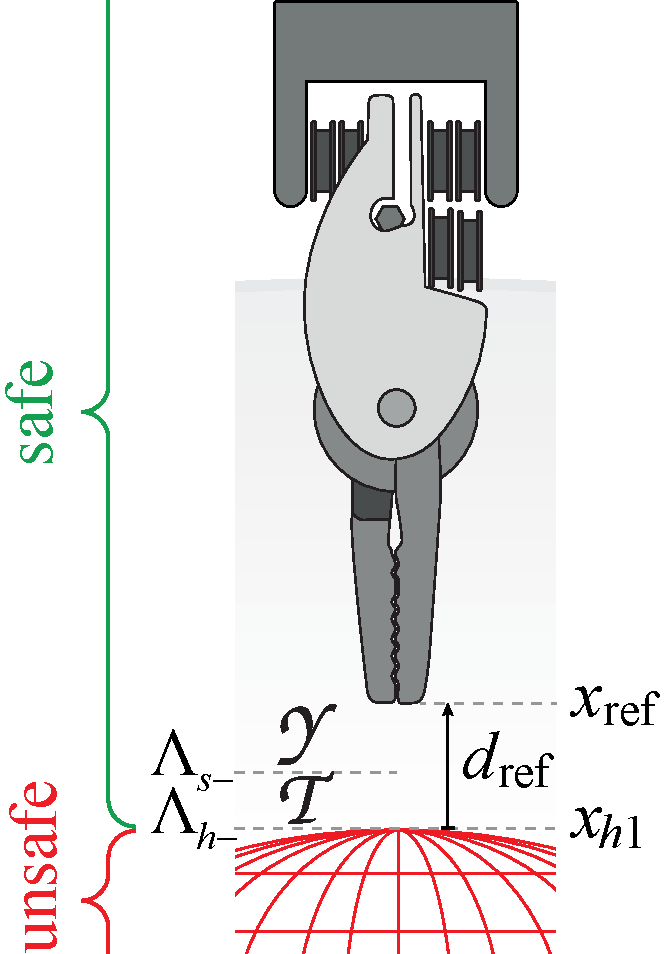
\includegraphics[width=0.175\linewidth]{dynamic_boundary_limits.pdf} \hspace*{0.4cm}
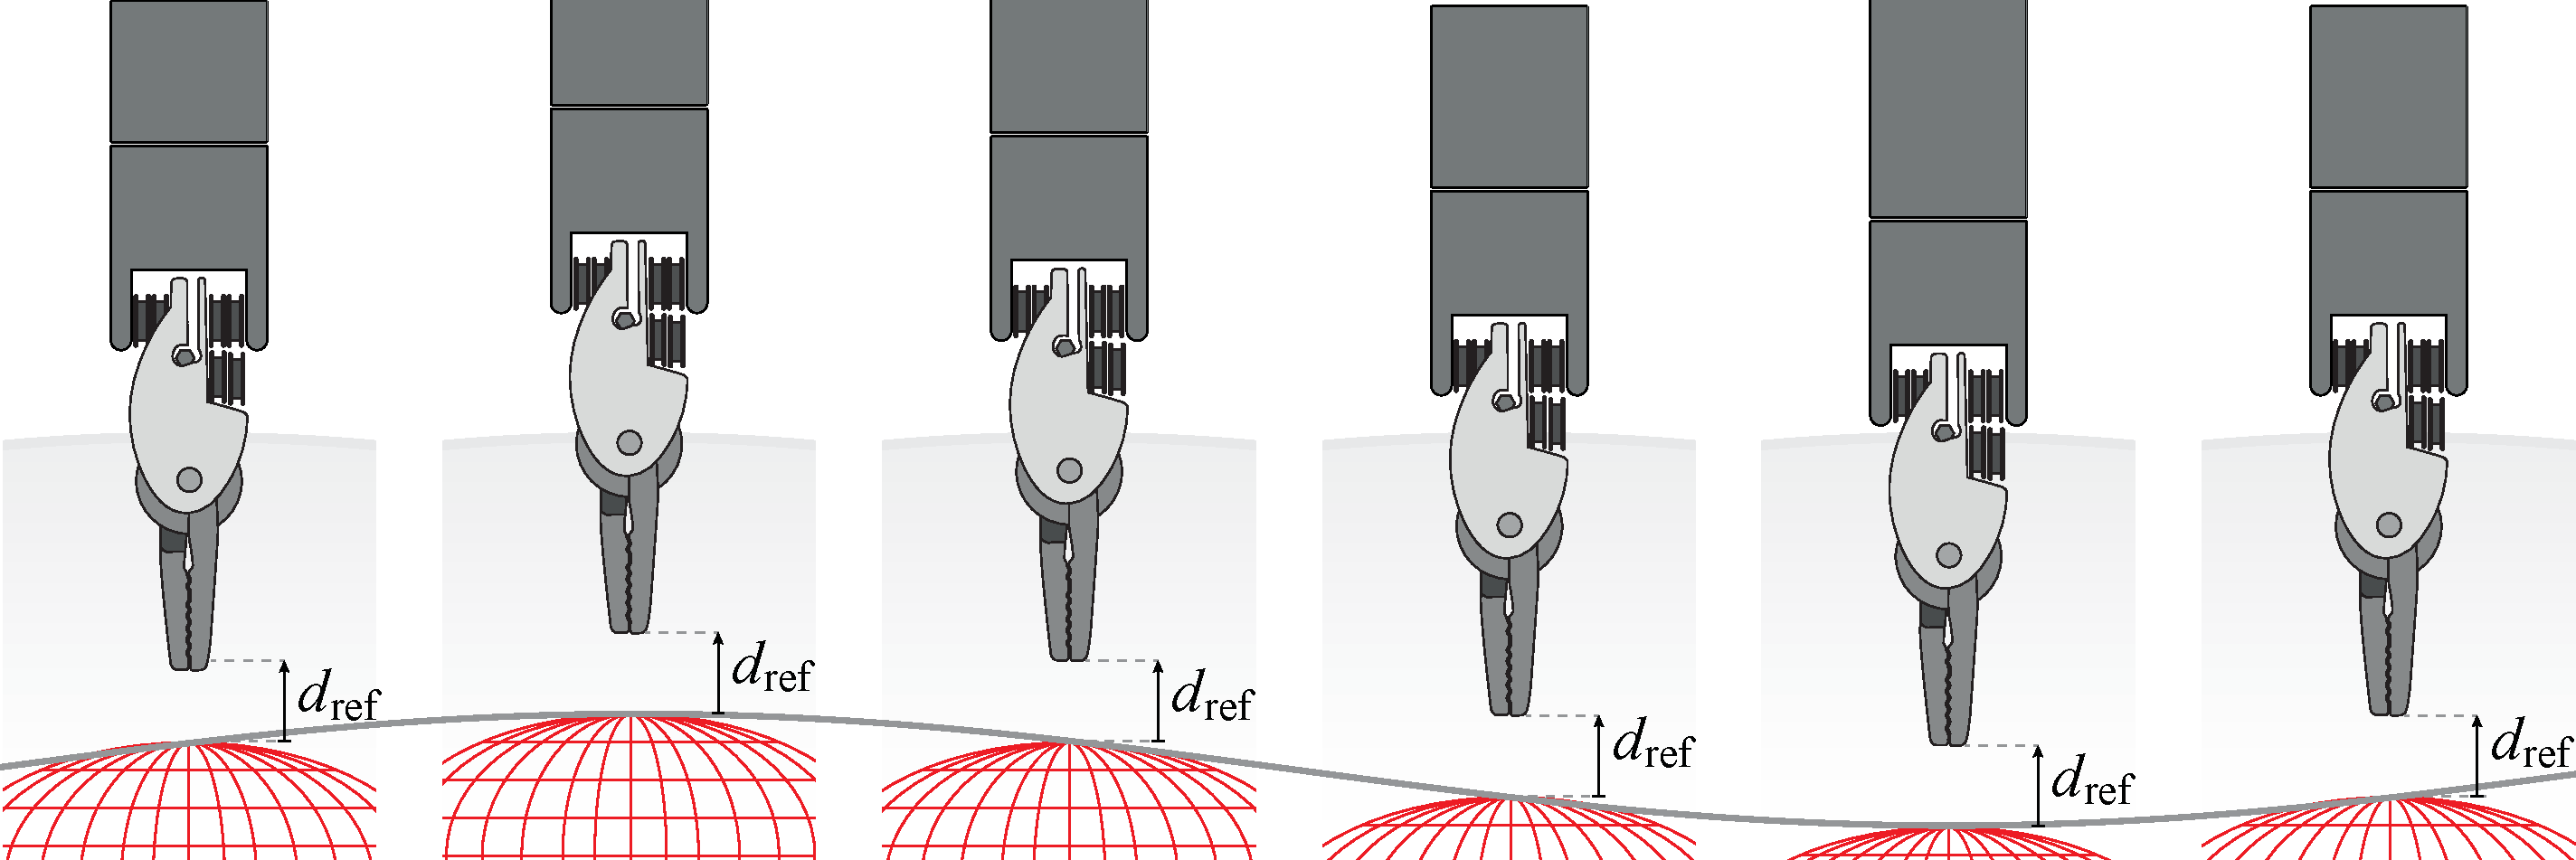
\includegraphics[width=0.75\linewidth]{dynamic_boundary_sequence.pdf}

\begin{minipage}{0.7\textwidth}
\scriptsize
\begin{align*}
& \dot{\textbf{x}} = \begin{bmatrix}
-1/\tau & 0 & 0 & 0 \\
0 & 0 & \omega_h & 0 \\
0 & -\omega_h & 0 & 0 \\
0 & 0 & 0 & 0
\end{bmatrix} \begin{bmatrix}
x_1 \\ x_{h1} \\ x_{h2} \\ d_\text{ref}
\end{bmatrix} + \begin{bmatrix}
1/\tau \\ 0 \\ 0 \\ 0
\end{bmatrix} u \\
&  u = \bar{N} x_\text{ref} - \textbf{K} x_1 = \bar{N}\Big( x_{h1} - x_1 \Big) - \textbf{K} x_1 = \bar{\textbf{K}}x
\end{align*}
\end{minipage}
\hspace*{0.1cm}
\begin{minipage}{0.25\textwidth}
\vspace*{0.2cm}

\includegraphics[width=0.75\linewidth]{barrier.jpg}
\hspace*{-0.3cm}
\vspace*{-0.2cm} \scriptsize
\begin{align*}
B(x) = \tilde{c}\Big( x_{h1} - x_1 \Big){\color{white}{lol}}
\end{align*}
\end{minipage}
\end{frame}

\begin{frame}{Sikkerhed for et dynamisk system}{Resultater}
\hspace*{-0.5cm}
\begin{minipage}{0.46\textwidth}
	\begin{itemize}
		\item Simulering
	\end{itemize}
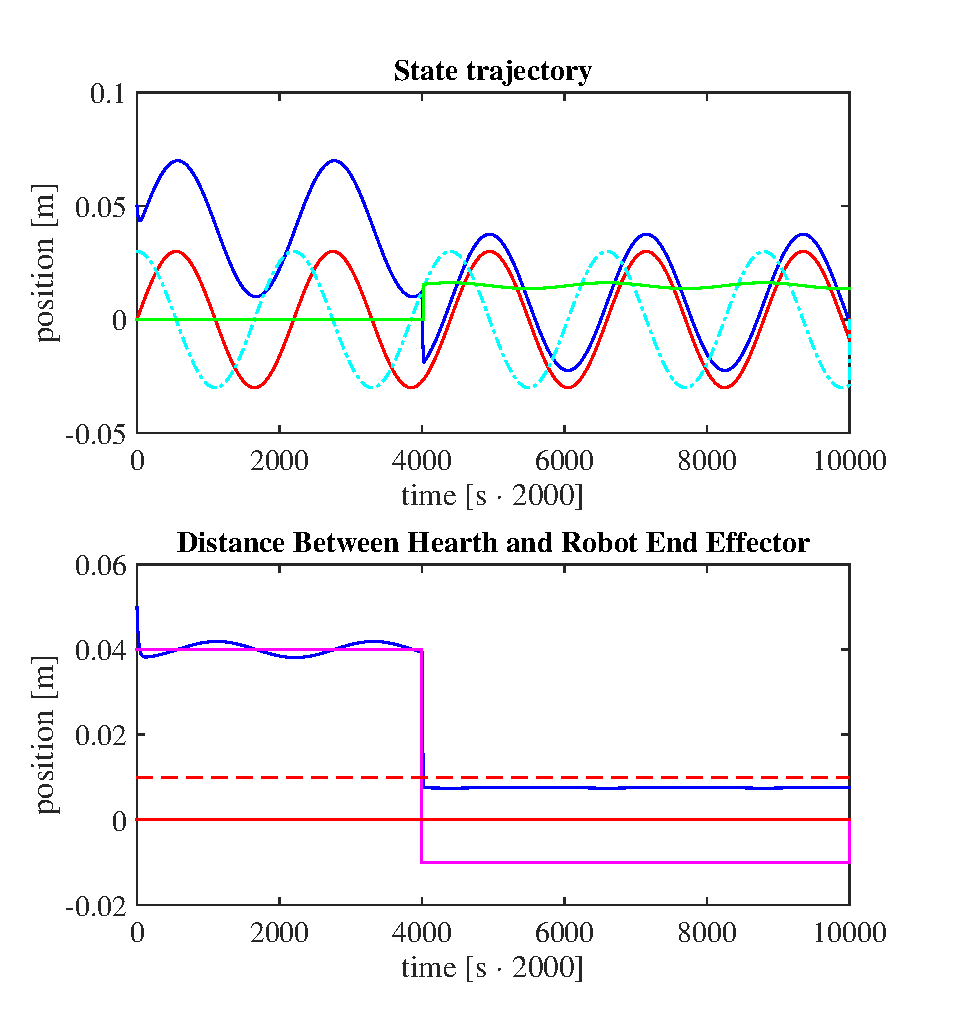
\includegraphics[width=1.17\linewidth]{dyn.eps}
\end{minipage}
\hspace{0.4cm}
\begin{minipage}{0.46\textwidth}
	\begin{itemize}
		\item Implementering
	\end{itemize}
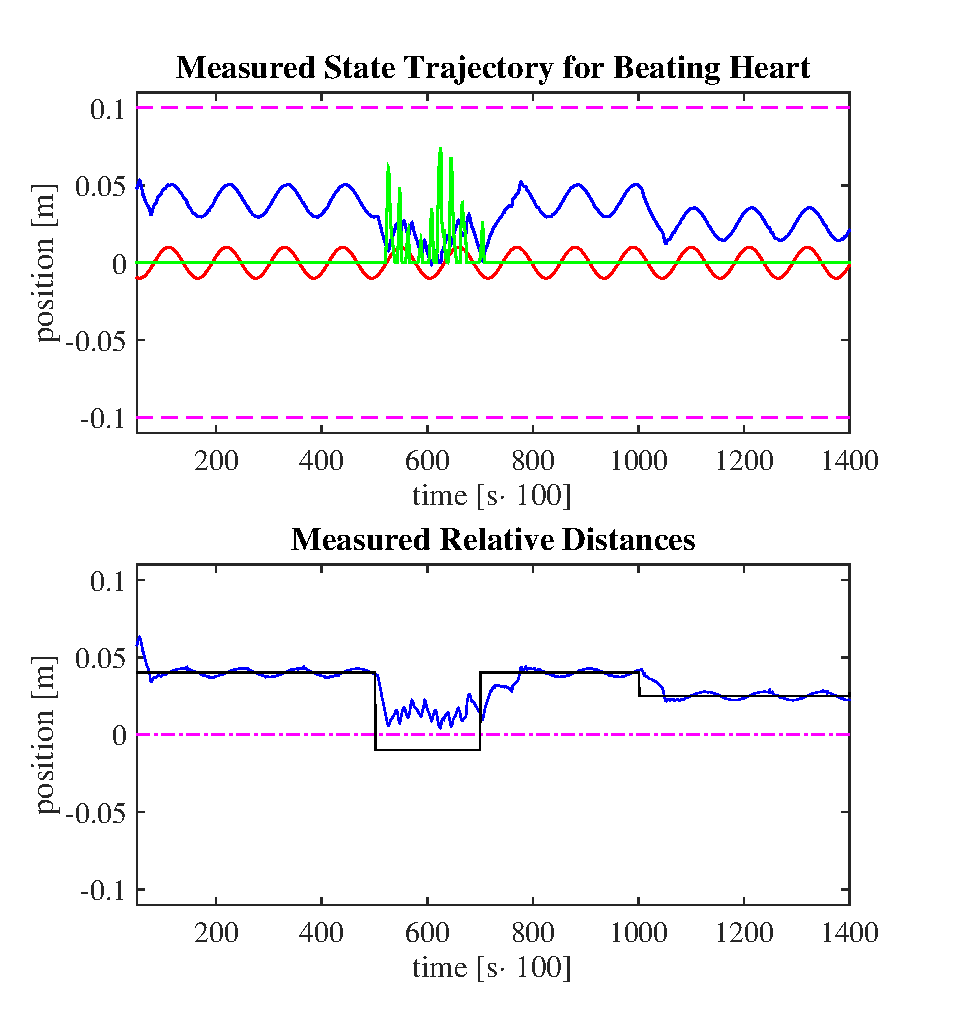
\includegraphics[width=1.17\linewidth]{dyn_meas.eps}
\end{minipage}

\end{frame}

\begin{frame}{Sikkerhed i det 3 dimensionelle rum}{På vej mod noget brugbart}
\section{Sikkerhed i 3D}
\vspace*{0.5cm}
\begin{itemize}
	\item Linear model hvor \textit{x, y} og \textit{z} er uafhænginge
	\item Kontrol topologi er identisk med 1D systemet
	\item Kortlægge og modifisere den kinematiske kæde
	\item Anvende kinematiske solvere (KDL)
	\item Definere CBF i 3D
\end{itemize}
\vspace*{-0.5cm}
\begin{minipage}{0.45\textwidth}
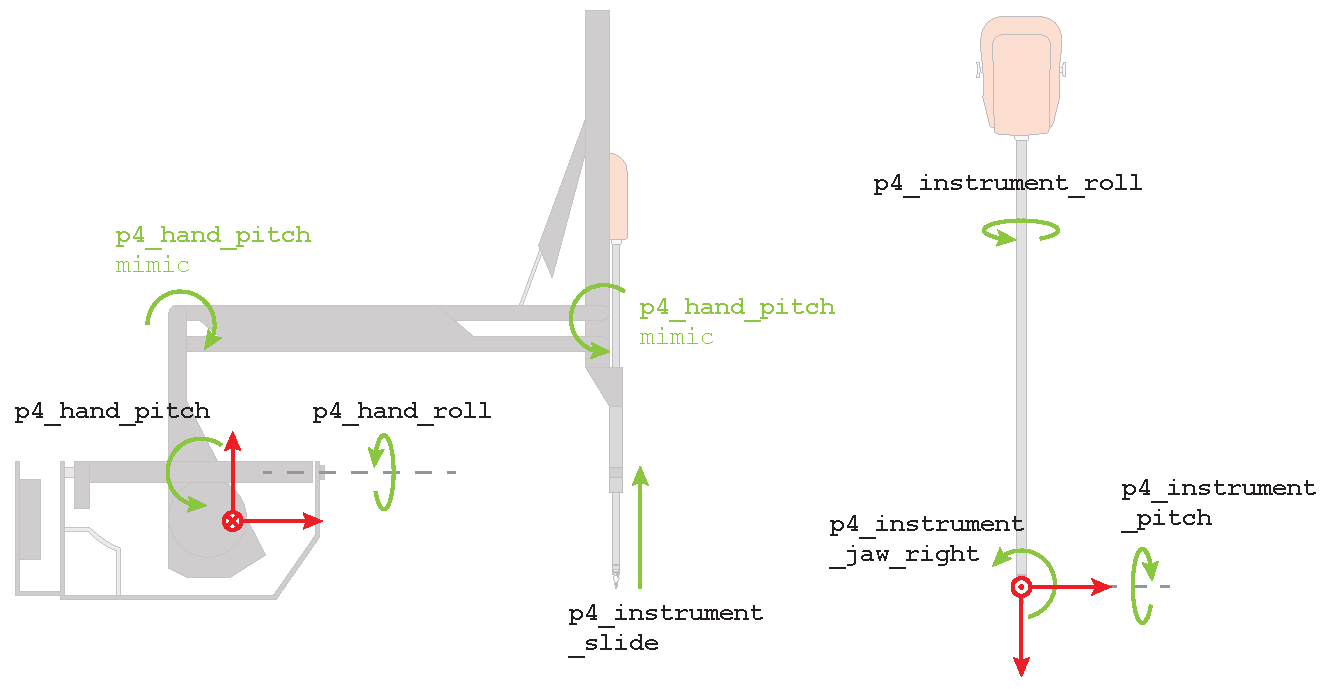
\includegraphics[width=1.2\linewidth]{simple_kinematics.pdf}
\end{minipage}
\hspace*{0.8cm}
\begin{minipage}{0.45\textwidth}
\includegraphics[width=1\linewidth]{3d_bar_ny.eps}
\end{minipage}
\end{frame}

\begin{frame}{Sikkerhed i det 3 dimensionelle rum}{Resultater}
\vspace*{0.4cm}
\hspace*{-0.2cm}
\begin{minipage}{0.46\textwidth}
\begin{itemize}
	\item Simulering
\end{itemize}
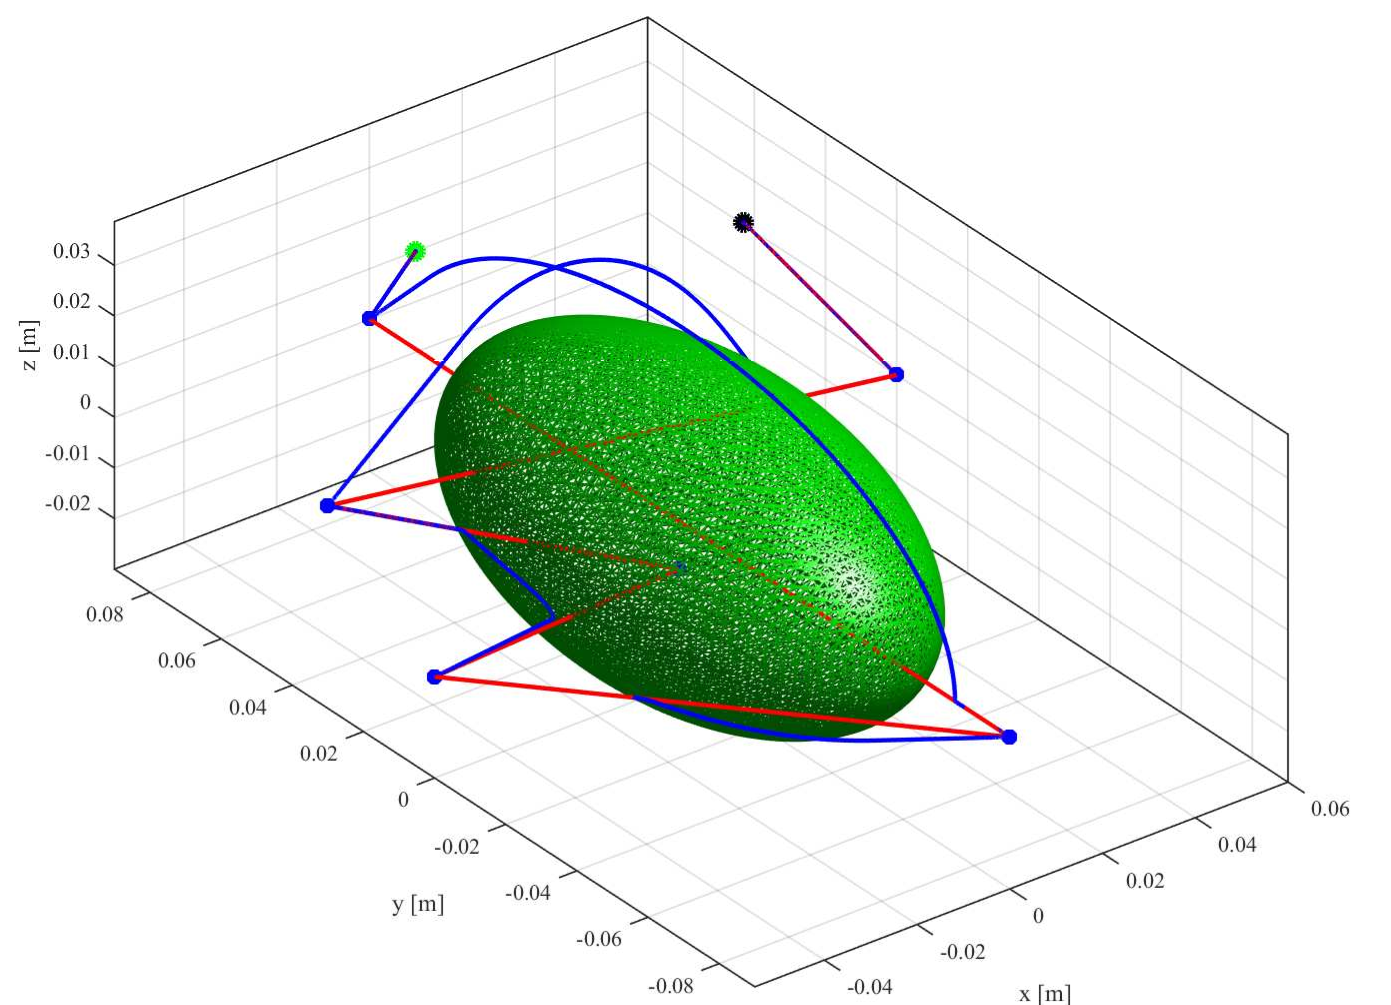
\includegraphics[width=1.0\linewidth]{traj_3d_1_sim.pdf}
\begin{itemize}
	\item Finder setpoints i $\mathcal{X}_0$
	\item Undgår $\mathcal{X}_u$ selvom setpoint er sikker
	\item Finder steady state i nærmeste sikre område
\end{itemize}
\end{minipage}
\hspace{0.2cm}
\begin{minipage}{0.46\textwidth}
\begin{itemize}
	\item Implementering
\end{itemize}
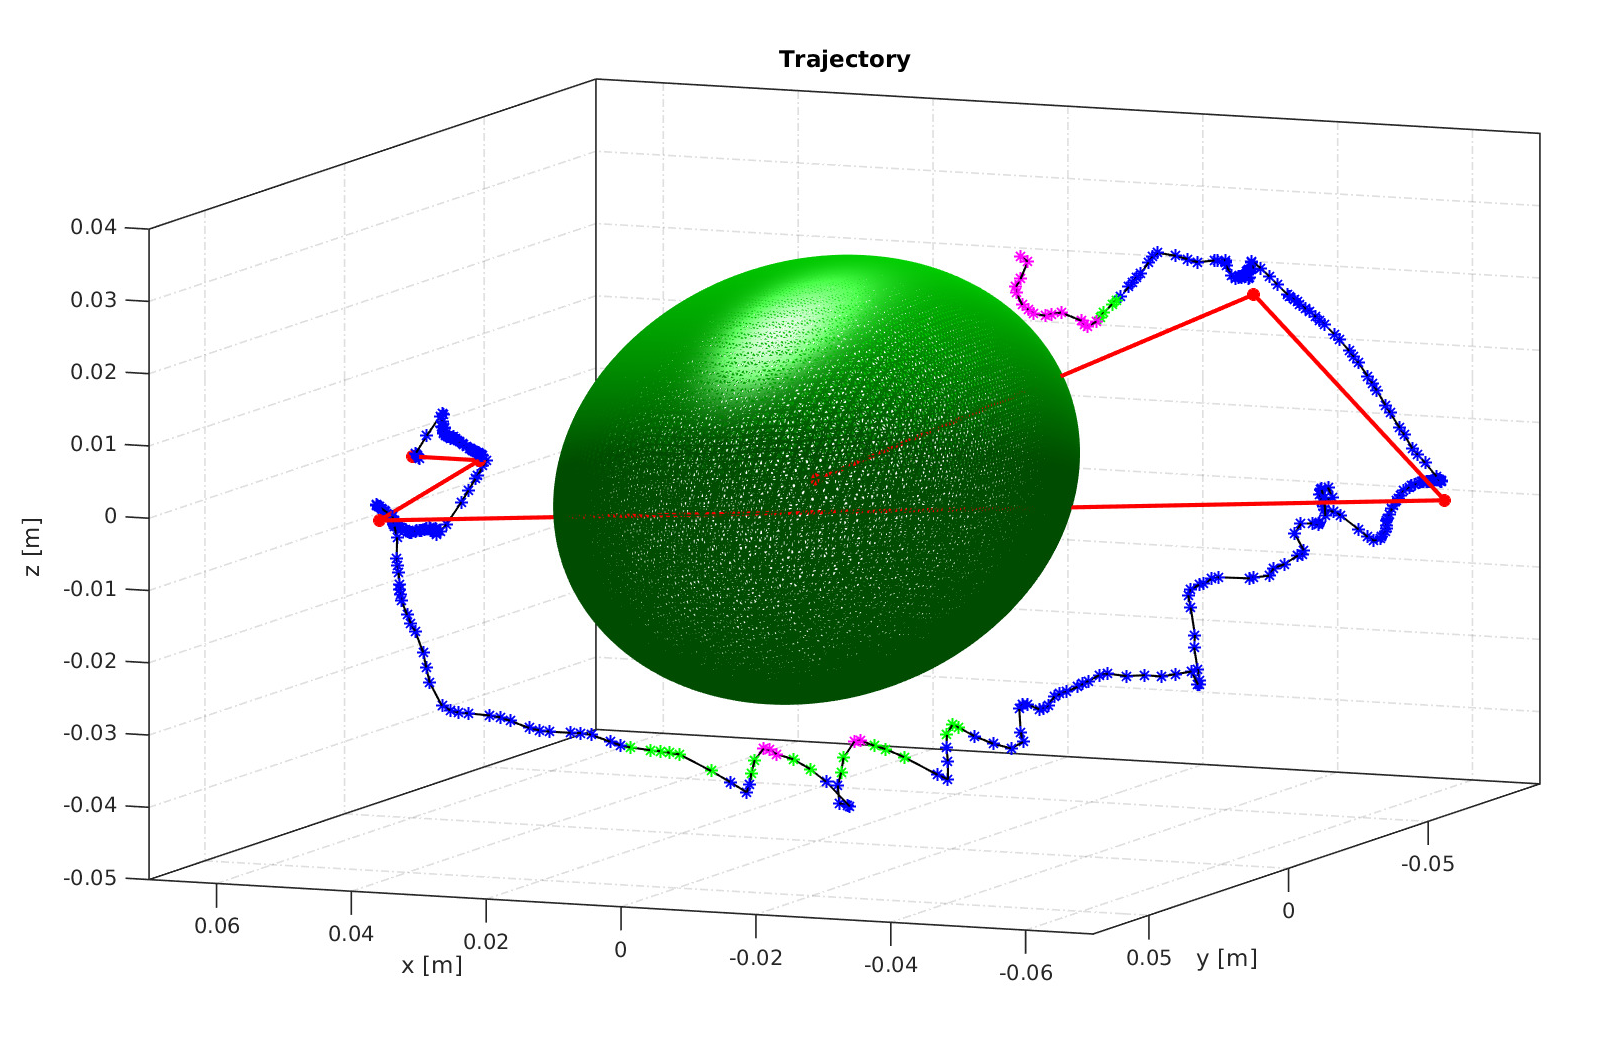
\includegraphics[width=1.1\linewidth]{traj_3d_meas-eps-converted-to.pdf}
\begin{itemize}
	\item Samme karakteristik som simulering
	\item En smule upræcis
	\item IK-solver finder ulogisk løsning - dog en løsning
\end{itemize}
\end{minipage}
\end{frame}
